\documentclass[tikz,border=10pt]{standalone}
\usetikzlibrary{arrows,intersections}
\begin{document}
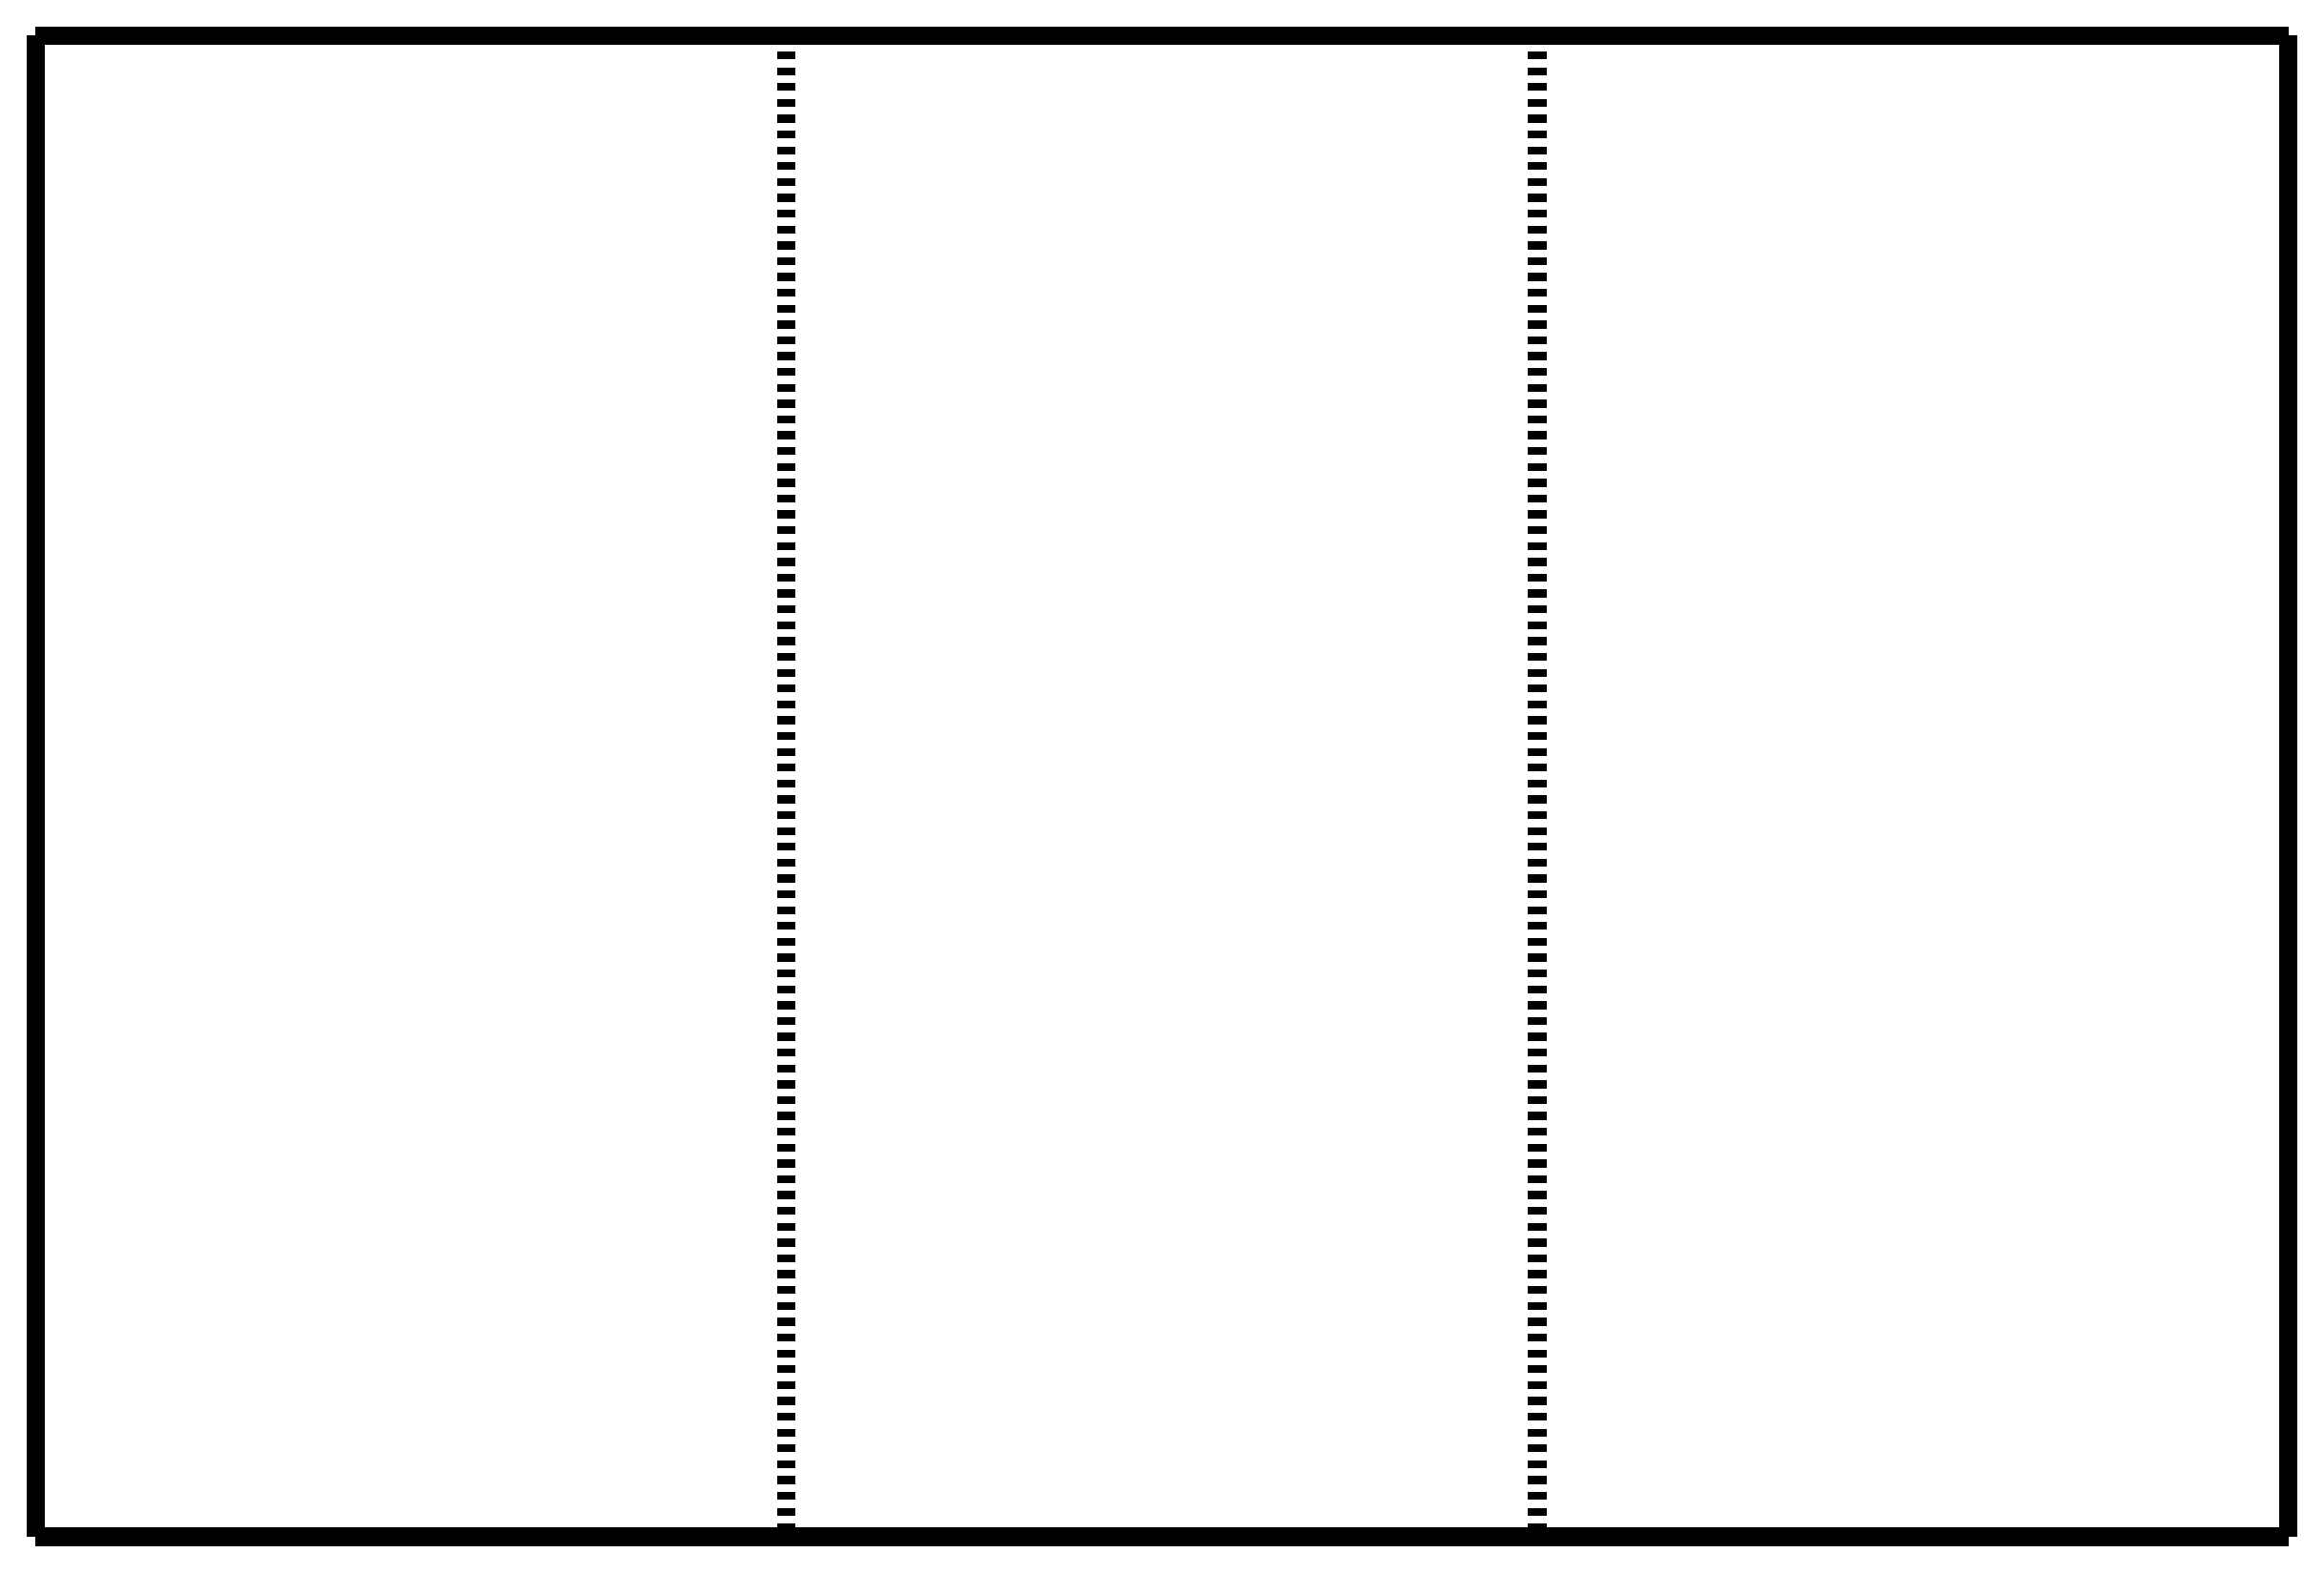
\begin{tikzpicture}[
    thick,
    >=stealth',
    dot/.style = {
      draw,
      fill = white,
      circle,
      inner sep = 0pt,
      minimum size = 4pt
    }
  ]
  \coordinate (O) at (0,0);
  \scope[]
	\draw[black, line width=7] plot[] coordinates {(0,0) (0,20)};
	\draw[black, line width=7] plot[] coordinates {(0,20) (30,20)};
	\draw[black, line width=7] plot[] coordinates {(30,20) (30,0)};
	\draw[black, line width=7] plot[] coordinates {(30,0) (0,0)};
	
	\draw[black, line width=7, /tikz/dashed] plot[] coordinates {(10,20) (10,0)};
	\draw[black, line width=7, /tikz/dashed] plot[] coordinates {(20,20) (20,0)};
    
  \endscope
\end{tikzpicture}
\end{document}